                
% ----------------------------------------------------------------------
%                   LATEX TEMPLATE FOR PhD THESIS
% ----------------------------------------------------------------------

% based on Harish Bhanderi's PhD/MPhil template, then Uni Cambridge
% http://www-h.eng.cam.ac.uk/help/tpl/textprocessing/ThesisStyle/
% corrected and extended in 2007 by Jakob Suckale, then MPI-CBG PhD programme
% and made available through OpenWetWare.org - the free biology wiki


%: Style file for Latex
% Most style definitions are in the external file PhDthesisPSnPDF.
% In this template package, it can be found in ./Latex/Classes/
\documentclass[twoside,11pt,table,xcdraw]{Latex/Classes/PhDthesisPSnPDF}

\usepackage[utf8]{inputenc}
\usepackage[english]{babel}
\usepackage{lipsum}  

%: Macro file for Latex
% Macros help you summarise frequently repeated Latex commands.
% Here, they are placed in an external file /Latex/Macros/MacroFile1.tex
% An macro that you may use frequently is the figuremacro (see introduction.tex)
%% This file contains macros that can be called up from connected TeX files
% It helps to summarise repeated code, e.g. figure insertion (see below).

% insert a centered figure with caption and description
% parameters 1:filename, 2:title, 3:description and label
\newcommand{\figuremacro}[3]{
	\begin{figure}[htbp]
		\centering
		\includegraphics[width=1\textwidth]{#1}
		\caption[#2]{\textbf{#2} - #3}
		\label{#1}
	\end{figure}
}

% insert a centered figure with caption and description AND WIDTH
% parameters 1:filename, 2:title, 3:description and label, 4: textwidth
% textwidth 1 means as text, 0.5 means half the width of the text
\newcommand{\figuremacroW}[4]{
	\begin{figure}[htbp]
		\centering
		\includegraphics[width=#4\textwidth]{#1}
		\caption[#2]{\textbf{#2} - #3}
		\label{#1}
	\end{figure}
}

% inserts a figure with wrapped around text; only suitable for NARROW figs
% o is for outside on a double paged document; others: l, r, i(inside)
% text and figure will each be half of the document width
% note: long captions often crash with adjacent content; take care
% in general: above 2 macro produce more reliable layout
\newcommand{\figuremacroN}[3]{
	\begin{wrapfigure}{o}{0.5\textwidth}
		\centering
		\includegraphics[width=0.48\textwidth]{#1}
		\caption[#2]{{\small\textbf{#2} - #3}}
		\label{#1}
	\end{wrapfigure}
}

% predefined commands by Harish
\newcommand{\PdfPsText}[2]{
  \ifpdf
     #1
  \else
     #2
  \fi
}

\newcommand{\IncludeGraphicsH}[3]{
  \PdfPsText{\includegraphics[height=#2]{#1}}{\includegraphics[bb = #3, height=#2]{#1}}
}

\newcommand{\IncludeGraphicsW}[3]{
  \PdfPsText{\includegraphics[width=#2]{#1}}{\includegraphics[bb = #3, width=#2]{#1}}
}

\newcommand{\InsertFig}[3]{
  \begin{figure}[!htbp]
    \begin{center}
      \leavevmode
      #1
      \caption{#2}
      \label{#3}
    \end{center}
  \end{figure}
}


%%% Local Variables: 
%%% mode: latex
%%% TeX-master: "~/Documents/LaTeX/CUEDThesisPSnPDF/thesis"
%%% End: 




%: ----------------------------------------------------------------------
%:                  TITLE PAGE: name, degree,..
% ----------------------------------------------------------------------
% below is to generate the title page with crest and author name

%if output to PDF then put the following in PDF header
\ifpdf  
    \pdfinfo { /Title 
               /Creator (TeX)
               /Producer (pdfTeX)
               /Author (Ana Iglesias Molina ana.iglesiasm@upm.es)
               /CreationDate (D:YYYYMMDDhhmmss)  %format D:YYYYMMDDhhmmss
               /ModDate (D:YYYYMMDDhhmm)
               /Subject (xyz)
               /Keywords () }
    \pdfcatalog { /PageMode (/UseOutlines)
                  /OpenAction (fitbh)  }
\fi

  
\title{Devising an interoperable and governable environment of mapping languages for Knowledge Graph construction}

% ----------------------------------------------------------------------
% The section below defines www links/email for author and institutions
% They will appear on the title page of the PDF and can be clicked
\ifpdf
 
  \author{{\hspace{7mm} Ana Iglesias Molina}}
  \supervisor{Oscar Corcho}
	%
	
%  \cityofbirth{born in XYZ} % uncomment this if your university requires this
%  % If city of birth is required, also uncomment 2 sections in PhDthesisPSnPDF
%  % Just search for the "city" and you'll find them.
%  \collegeordept{{Programa de Doctorado de Inteligencia Artificial \\ Facultad de Inform\'atica}}  
%  \university{\href{http://www.upm.es}{Universidad Polit\'ecnica de Madrid}}  
  % The crest is a graphics file of the logo of your research institution.
  % Place it in ./0_frontmatter/figures and specify the width
%  \crest{
\includegraphics[width=3cm]{escudofi.pdf}}
\crest{  
		\centering
 		\begin{tabular}{l c}
			\multirow{3}{*}{
\includegraphics[width=2cm]{0_frontmatter/figures/escudofi.pdf}} & \\
			& \textbf{Programa de Doctorado de Inteligencia Artificial} \\ 
			& \textbf{Escuela T\'ecnica Superior de Ingenieros Inform\'aticos} \\
		\end{tabular}
}
% If you are not creating a PDF then use the following. The default is PDF.
\else
  \author{YourName}
%  \cityofbirth{born in XYZ}
  \collegeordept{CollegeOrDept}
  \university{University}
  \crest{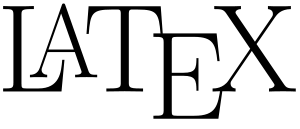
\includegraphics[width=4cm]{logo}}
\fi

%\renewcommand{\submittedtext}{change the default text here if needed}
\degree{Philosophi\ae Doctor (PhD), DPhil,..}
\degreedate{XXX, 2023}


% ----------------------------------------------------------------------
       
% turn of those nasty overfull and underfull hboxes
%\tolerance=1
%\emergencystretch=\maxdimen
%\hyphenpenalty=10000

\hbadness=10000
\hfuzz=50pt

\usepackage{enumitem}
\usepackage[table,xcdraw]{xcolor}
\usepackage{floatrow}
\usepackage{mathptmx}
\usepackage[T1]{fontenc}
\usepackage{textcomp}
\usepackage{listings}
\usepackage{tikz}
%\usepackage{paralist} 
\usepackage{import}

\usepackage{array}
\usepackage{color}
\usepackage{pgfplots}
\usepackage{amsmath}
\usepackage{xspace}
\usepackage{amssymb}
%\usepackage{enumerate}
%\usepackage{float}
%\usepackage{algpseudocode}
%\usepackage{algorithm}
\usepackage{verbatim}
\usepackage{multirow}
\usepackage{siunitx}
\usepackage{url}
\usepackage{chngcntr}
\usepackage{amsthm}
\usepackage{latexsym}
\usepackage{subfig}
\usepackage{pifont}
\usepackage{graphicx}
\usepackage{caption}
\usepackage{adjustbox} 
\usepackage{rotating}
%\usepackage{subcaption}
%\captionsetup{compatibility=false}
\usepackage{bibentry}
\usepackage{mathtools}
\usepackage{algorithm}
\usepackage{algorithmic}

\usepackage{ctable}

\usepackage[htt]{hyphenat}
\usetikzlibrary{patterns}
\counterwithout{footnote}{chapter}


%%<ALVARO>

\newcommand*\rot{\rotatebox{75}}
\newcommand*\OK{\ding{51}}
\newcommand{\argmax}[1]{\underset{#1}{\operatorname{arg}\,\operatorname{max}}\;}
\DeclarePairedDelimiter\ceil{\lceil}{\rceil}
\DeclarePairedDelimiter\floor{\lfloor}{\rfloor}

\newcounter{groupcount}
\pgfplotsset{
    draw group line/.style n args={5}{
        after end axis/.append code={
            \setcounter{groupcount}{0}
            \pgfplotstableforeachcolumnelement{#1}\of\datatable\as\cell{%
                \def\temp{#2}
                \ifx\temp\cell
                    \ifnum\thegroupcount=0
                        \stepcounter{groupcount}
                        \pgfplotstablegetelem{\pgfplotstablerow}{[index]0}\of\datatable
                        \coordinate [yshift=#4] (startgroup) at (axis cs:\pgfplotsretval,0);
                    \else
                        \pgfplotstablegetelem{\pgfplotstablerow}{[index]0}\of\datatable
                        \coordinate [yshift=#4] (endgroup) at (axis cs:\pgfplotsretval,0);
                    \fi
                \else
                    \ifnum\thegroupcount=1
                        \setcounter{groupcount}{0}
                        \draw [
                            shorten >=-#5,
                            shorten <=-#5
                        ] (startgroup) -- node [anchor=north] {#3} (endgroup);
                    \fi
                \fi
            }
            \ifnum\thegroupcount=1
                        \setcounter{groupcount}{0}
                        \draw [
                            shorten >=-#5,
                            shorten <=-#5
                        ] (startgroup) -- node [anchor=north] {#3} (endgroup);
            \fi
        }
    }
}




%%<IDAFEN>
\usepackage{xcolor}
\usepackage{color}
\definecolor{mygray}{rgb}{0.5,0.5,0.5}
\newcommand{\dfp}{dispel4py}

%\lstset{
%	basicstyle=\footnotesize,
%	breakatwhitespace=true,
%	breaklines=true,
%	numberstyle=\tiny\color{mygray},
%	numbers=left,
%	xleftmargin=1.5em,
%	frame=single,
%	framexleftmargin=1em,
%	frame=bt,
%}

%%subindex


\usepackage{multirow}

%%highlighting package
\usepackage{color}\newcommand{\mynote}[2][inline]{\color{red} [PENDING]: #2\color{black}}

%\newcommand{\mymark}[1]{\colorbox{orange}{#1}}
\newcommand{\mymark}[2][inline]{\color{orange}#2\color{black}}
\newcommand{\new}[2][inline]{\color{black}#2\color{black}}
\newcommand{\newtwo}[2][inline]{\color{black}#2\color{black}}
%\newcommand{\mynote}[2][inline]{\color{red} [PENDING]: #2\color{black}}
\usepackage{epigraph}
%%adding subsubsections
%\setcounter{secnumdepth}{3}

%%</IDAFEN>

\DeclareCaptionFormat{algor}{%
  \hrulefill\par\offinterlineskip\vskip1pt%
    \textbf{#1#2}#3\offinterlineskip\hrulefill}
\DeclareCaptionStyle{algori}{singlelinecheck=off,format=algor,labelsep=space}
%\captionsetup[algorithm]{style=algori}

\pdfoptionpdfminorversion 6

%% PIERRE

\definecolor{s1}{RGB}{228, 26, 28}
\definecolor{s2}{RGB}{55, 126, 184}
\definecolor{s3}{RGB}{77, 175, 74}
\definecolor{s4}{RGB}{152, 78, 163}
\definecolor{s5}{RGB}{255, 127, 0}
\definecolor{s6}{RGB}{160, 82, 45}

\pgfplotscreateplotcyclelist{tyr}{%
    s1,every mark/.append style={fill=white},mark=*\\%
    s2,every mark/.append style={fill=white},mark=square*\\%
    s3,every mark/.append style={fill=white},mark=diamond*\\%
    s4,every mark/.append style={fill=white},mark=triangle*\\%
    s5,every mark/.append style={fill=white},mark=pentagon*\\%
    s6,every mark/.append style={fill=white},mark=otimes*\\%
}

\pgfplotsset{compat=1.11,
    /pgfplots/ybar legend/.style={
    /pgfplots/legend image code/.code={%
       \draw[##1,/tikz/.cd,yshift=-0.25em]
        (0cm,0cm) rectangle (6.5pt,0.7em);},
   },
}

\pgfplotsset{
    grid=major,
    width=9cm,
    height=6cm,
    compat=1.9
}

\makeatletter
\g@addto@macro\@floatboxreset\centering
\makeatother

\pgfplotsset{plot coordinates/math parser=false}


\makeatletter
\pgfplotsset{
    groupplot xlabel/.initial={},
    every groupplot x label/.style={
        at={($({group c1r\pgfplots@group@rows.west}|-{group c1r\pgfplots@group@rows.outer south})!0.5!({group c\pgfplots@group@columns r\pgfplots@group@rows.east}|-{group c\pgfplots@group@columns r\pgfplots@group@rows.outer south})$)},
        anchor=north,
    },
    groupplot ylabel/.initial={},
    every groupplot y label/.style={
            rotate=90,
        at={($({group c1r1.north}-|{group c1r1.outer
west})!0.5!({group c1r\pgfplots@group@rows.south}-|{group c1r\pgfplots@group@rows.outer west})$)},
        anchor=south
    },
    execute at end groupplot/.code={%
      \node [/pgfplots/every groupplot x label]
{\pgfkeysvalueof{/pgfplots/groupplot xlabel}};  
      \node [/pgfplots/every groupplot y label] 
{\pgfkeysvalueof{/pgfplots/groupplot ylabel}};  
    },
    group/only outer labels/.style =
{
group/every plot/.code = {%
    \ifnum\pgfplots@group@current@row=\pgfplots@group@rows\else%
        \pgfkeys{xticklabels = {}, xlabel = {}}\fi%
    \ifnum\pgfplots@group@current@column=1\else%
        \pgfkeys{yticklabels = {}, ylabel = {}}\fi%
}
}
}

\def\endpgfplots@environment@groupplot{%
    \endpgfplots@environment@opt%
    \pgfkeys{/pgfplots/execute at end groupplot}%
    \endgroup%
}
\makeatother

\definecolor{gray}{rgb}{0.95,0.95,0.95}

\usetikzlibrary{arrows, positioning, shapes.multipart, calc, fit, patterns, decorations.text,
decorations.pathreplacing, shapes.symbols}
\usepgfplotslibrary{groupplots}

%% Tables

\newcommand{\specialcell}[2][c]{%
  \begin{tabular}[#1]{@{}c@{}}#2\end{tabular}}
  
\newcolumntype{P}[1]{>{\centering\arraybackslash}p{#1}}
\newcolumntype{M}[1]{>{\centering\arraybackslash}m{#1}}
\newcolumntype{N}{@{}m{0pt}@{}}

%% Algo

\renewcommand{\algorithmicrequire}{\textbf{Input:}}
\renewcommand{\algorithmicensure}{\textbf{Output:}}
\let\oldReturn\Return
%\renewcommand{\Return}{\State\oldReturn}
%\renewcommand{\algorithmicforall}{\textbf{for each}}

%\algnewcommand{\LineComment}[1]{\State{\textit{\textcolor{black!60}{\(\triangleright\) #1}}}}

%% PGF

\pgfdeclarelayer{bg}
\pgfdeclarelayer{mbg}
\pgfsetlayers{bg,mbg,main}

%% Sections

\newcommand{\lsection}[2]{
    \section{#2}
    \label{sec:#1}
}

\newcommand{\lsubsection}[2]{
    \subsection{#2}
    \label{sec:#1}
}

\newcommand{\lsubsubsection}[2]{
    \subsubsection{#2}
    \label{sec:#1}
}

\newcommand{\lsecref}[1]{\ref{sec:#1}}

\newcommand{\csubfloat}[2][]{%
  \makebox[0pt]{\subfloat[#1]{#2}}%
}
\newcommand{\centerhfill}[1][\quad]{\hspace{\stretch{0.5}}#1\hspace{\stretch{0.5}}}

\makeatletter
\newcommand\resetstackedplots{
\makeatletter
\pgfplots@stacked@isfirstplottrue
\makeatother
\addplot [forget plot,draw=none] coordinates{(1,0) (2,0) (3,0)};
}

%% /PIERRE

%: --------------------------------------------------------------
%:                  FRONT MATTER: dedications, abstract,..
% --------------------------------------------------------------

\begin{document}

%\language{english}

% sets line spacing
\renewcommand\baselinestretch{1.2}
\baselineskip=18pt plus1pt

\theoremstyle{plain}
\newtheorem{thm}{Theorem}[chapter] % reset theorem numbering for each chapter


\theoremstyle{definition}
\newtheorem{definition}[thm]{Definition} % definition numbers are dependent on theorem numbers

\newcommand{\attention}[1]{{\color{red}\textbf{#1}}}

\renewcommand\appendixname{ANNEX}


%: ----------------------- generate cover page ------------------------
\frontmatter
\maketitle  % command to print the title page with above variables


%: ----------------------- cover page back side ------------------------
% Your research institution may require reviewer names, etc.
% This cover back side is required by Dresden Med Fac; uncomment if needed.

% ALVARO: I'll have to change this

%\newpage
\pagestyle{plain}
\cleardoublepage
\pagestyle{plain}


\noindent Tribunal nombrado por el Sr. Rector Magfco. de la Universidad Polit\'{e}cnica de
Madrid, el d\'{i}a 9 de Junio de 2021. %\mynote{DD de YYYY de 2015}

\vspace{10mm}
Presidente:\hspace{0.3mm} TBDDr. Marcelo Arenas

\vspace{5mm}
Vocal: \hspace{6.7mm} TBDDr. Juan Sequeda 

\vspace{5mm}
Vocal: \hspace{6.7mm} TBDDrDra. Anastasia Dimou

\vspace{5mm}
Vocal: \hspace{6.7mm} TBDDrDr. Álvaro Sicilia Gómez 


\vspace{5mm}
Secretario:\hspace{0.67mm} TBDDrDr. Raúl García Castro

\vspace{5mm}
Suplente: \hspace{1.5mm} TBDDrDr. Mariano Fernández López   

\vspace{5mm}
Suplente: \hspace{1.5mm} TBDDrDr. Alberto Bugarín Díz

\vspace{10mm}
\noindent TBDDrRealizado el acto de defensa y lectura de la Tesis el d\'{i}a 28 de Junio de 2021 en la Escuela T\'ecnica Superior de Ingenieros Inform\'aticos

\vspace{5mm}
\noindent Calificaci\'{o}n: \rule{123mm}{0.2mm}
\vspace{20mm}

EL PRESIDENTE \hspace{30mm} VOCAL 1 \hspace{30mm} VOCAL 2

\vspace{30mm}
%\begin{center}
\hspace{15mm} VOCAL 3 \hspace{45mm} EL SECRETARIO
%\end{center}




%: ----------------------- tie in front matter ------------------------

%\frontmatter
\cleardoublepage
% Thesis Dedictation ---------------------------------------------------

\begin{dedication} %this creates the heading for the dedication page



\end{dedication}

% ----------------------------------------------------------------------
\cleardoublepage

\begin{acknowledgementslong} 


\end{acknowledgementslong}












%: ----------------------- abstract ------------------------

% Your institution may have specific regulations if you need an abstract and where it is to be placed in the document. The default here is just after title.
\cleardoublepage

% Thesis Abstract -----------------------------------------------------


\begin{abstractslong}    

\end{abstractslong}

\cleardoublepage
\begin{abstractslongSpanish}

\end{abstractslongSpanish}
% ---------------------------------------------------------------------- 


% The original template provides and abstractseparate environment, if your institution requires them to be separate. I think it's easier to print the abstract from the complete thesis by restricting printing to the relevant page.
% \begin{abstractseparate}
%   
% Thesis Abstract -----------------------------------------------------


\begin{abstractslong}    

\end{abstractslong}

\cleardoublepage
\begin{abstractslongSpanish}

\end{abstractslongSpanish}
% ---------------------------------------------------------------------- 

% \end{abstractseparate}


%: ----------------------- contents ------------------------
\cleardoublepage
\setcounter{secnumdepth}{3} % organisational level that receives a numbers
\setcounter{tocdepth}{2}    % print table of contents for level 3
\tableofcontents           % print the table of contents
% levels are: 0 - chapter, 1 - section, 2 - subsection, 3 - subsection


%: ----------------------- list of figures/tables ------------------------

\listoffigures	% print list of figures

\listoftables  % print list of tables

\listofalgorithms % Print list of algorithms


%: ----------------------- glossary ------------------------

% Tie in external source file for definitions: /0_frontmatter/glossary.tex
% Glossary entries can also be defined in the main text. See glossary.tex

%% this file is called up by thesis.tex
% content in this file will be fed into the main document

% Glossary entries are defined with the command \nomenclature{1}{2}
% 1 = Entry name, e.g. abbreviation; 2 = Explanation
% You can place all explanations in this separate file or declare them in the middle of the text. Either way they will be collected in the glossary.

% required to print nomenclature name to page header
\markboth{\MakeUppercase{\nomname}}{\MakeUppercase{\nomname}}


% ----------------------- contents from here ------------------------

% chemicals
%\nomenclature{DAPI}{4',6-diamidino-2-phenylindole; a fluorescent stain that binds strongly to DNA and serves to marks the nucleus in fluorescence microscopy} 
%\nomenclature{DEPC}{diethyl-pyro-carbonate; used to remove RNA-degrading enzymes (RNAases) from water and laboratory utensils}
%\nomenclature{DMSO}{dimethyl sulfoxide; organic solvent, readily passes through skin, cryoprotectant in cell culture}
%\nomenclature{EDTA}{Ethylene-diamine-tetraacetic acid; a chelating (two-pronged) molecule used to sequester most divalent (or trivalent) metal ions, such as calcium (Ca$^{2+}$) and magnesium (Mg$^{2+}$), copper (Cu$^{2+}$), or iron (Fe$^{2+}$ / Fe$^{3+}$)}



 
%
%\begin{multicols}{2} % \begin{multicols}{#columns}[header text][space]
%\begin{footnotesize} % scriptsize(7) < footnotesize(8) < small (9) < normal (10)
%
%\printnomenclature[1.5cm] % [] = distance between entry and description
%\label{nom} % target name for links to glossary
%
%\end{footnotesize}
%\end{multicols}



%: --------------------------------------------------------------
%:                  MAIN DOCUMENT SECTION
% --------------------------------------------------------------

% the main text starts here with the introduction, 1st chapter,...
\mainmatter

%\renewcommand{\chaptername}{} % uncomment to print only "1" not "Chapter 1"
%\titleformat{\chapter}[display]{\normalfont\bfseries\}{\chaptertitlename\ \thechapter}{5pt}{\Huge}

%-#####-> Uncomment to have Andres' style for chapter title

%\titleformat{\chapter}[display]
%{\bfseries\Large}
%{\filleft\MakeUppercase{\chaptertitlename} \Huge\thechapter}
%{4ex}
%{\titlerule
%\vspace{2ex}%
%\filright}
%[\vspace{2ex}%
%\titlerule]

%-#####-> End uncomment


\chapter{Introduction}
\label{chap:intro}






\chapter{State of the Art}
\label{chap:sota}


\chapter{Objectives and Contributions}
\label{chap:objectives}



\chapter{Definition, study and abstraction of mappings and mapping rules}
\label{chapter:mappigs}



\chapter{Enhancing the creation of mapping rules}
\label{chapter:creation}



\chapter{Maintenance of KGs, reframing or recreating?}
\label{chapter:reframing}




\chapter{Governing Knowledge Graphs}
\label{chapter:governance}


\chapter{Conclusions and Future work}
\label{chap:conc}


\appendix
%\chapter{Mapeathor Mappings}
\label{sec:appendix-mapeathor}

\begin{captionedlisting}{lst:chp5-1_rml-output}{RML mapping generated with Mapeathor from the spreadsheet shown in Tables \ref{tab:chp5-1_prefix_sheet}, \ref{tab:chp5-1_subject_sheet}, \ref{tab:chp5-1_source_sheet}, \ref{tab:chp5-1_po_sheet} and \ref{tab:chp5-1_function_sheet}. }
\centering
{\begin{lstlisting}[numbers=left,basicstyle=\ttfamily\small,columns=flexible]
@prefix rr: <http://www.w3.org/ns/r2rml#>.
@prefix xsd: <http://www.w3.org/2001/XMLSchema#>.
@prefix rml: <http://semweb.mmlab.be/ns/rml#>.
@prefix ql: <http://semweb.mmlab.be/ns/ql#>.
@prefix rdf: <http://www.w3.org/1999/02/22-rdf-syntax-ns#>.
@prefix ex: <http://ex.com/>.
@prefix grel: <http://semweb.datasciencelab.be/ns/grel#>.
@base <http://example.com/>.

<#PERSON>
    a rr:TriplesMap;
    rml:logicalSource [
    	rml:source "/home/user/data/people.csv";
    	rml:referenceFormulation ql:CSV;
    ];
    rr:subjectMap [
    	a rr:Subject ;
    	rr:termType rr:IRI ;
    	rr:template "http://ex.com/Person/{name}" ;
    	rr:class ex:Person ;
    	rr:class ex:Athlete ;
    ];
    rr:predicateObjectMap [
    	rr:predicateMap	[ rr:constant ex:name];
    	rr:objectMap	[ rml:reference "name"; 
                      rr:termType rr:Literal;  
                      rr:datatype xsd:string;  
                      rr:language "en" ]
    ];
    rr:predicateObjectMap [
    	rr:predicateMap	[ rr:constant ex:plays ];
    	rr:objectMap	[
    		rr:parentTriplesMap	<#SPORT>;
    		rr:joinCondition	[
    			rr:child	"sport_id";
    			rr:parent	"id";
    		];
    	];
    ];
    rr:predicateObjectMap [
      rr:predicateMap	[ rr:constant ex:birthdate] ;
      rr:objectMap	[
    	  rml:functionExecution <#Fun-date> ;
    	  rml:return grel:dateOut ;
    	];
    ]; .

<#SPORT>
    a rr:TriplesMap;
    rml:logicalSource [
    	rml:source "/home/user/data/sports.json";
    	rml:referenceFormulation ql:JSONPath;
        rml:iterator "$\dollar$.*";
    ];
    rr:subjectMap [
    	a rr:Subject ;
    	rr:termType rr:IRI ;
    	rr:template "http://ex.com/Sport/{sport}" ;
    	rr:class ex:Sport ;
    	rr:graphMap [ rr:constant "ex:SportsGraph" ] ;
    ];
    rr:predicateObjectMap [
    	rr:predicateMap	[ rr:constant ex:name];
    	rr:objectMap	[ rml:reference "sport";  
                      rr:termType rr:Literal;  
                      rr:datatype xsd:string;  
                      rr:language "en" ]
    ];
    rr:predicateObjectMap [
    	rr:predicateMap	[ rr:constant ex:code];
    	rr:objectMap	[ rml:reference "id";  
                      rr:termType rr:Literal;  
                      rr:datatype xsd:integer ]
    ]; .

<#Fun-date> a rml:FunctionExecution;
    rml:function grel:toDate ;
    rml:input [
      a rml:Input ;
      rml:parameter grel:valueParam1 ;
      rml:inputValueMap [ rml:reference "birthdate" ];
    ];
    rml:input [
      a rml:Input ;
      rml:parameter grel:valueParam2 ;
      rml:inputValueMap [ rr:constant "dd/MM/yyyy" ];
    ];
    rml:input [
      a rml:Input ;
      rml:parameter grel:valueParam3 ;
      rml:inputValueMap [ rr:constant "yyyy-MM-dd" ];
    ]; .
\end{lstlisting}}
\end{captionedlisting}

\begin{captionedlisting}{lst:chp5-1_r2rml-output}{R2RML mapping generated with Mapeathor from the spreadsheet shown in Tables \ref{tab:chp5-1_prefix_sheet}, \ref{tab:chp5-1_subject_sheet}, \ref{tab:chp5-1_source_sheet}, \ref{tab:chp5-1_po_sheet} and \ref{tab:chp5-1_function_sheet}. }
\centering
{\begin{lstlisting}[numbers=left,basicstyle=\ttfamily\small,columns=flexible]
@prefix rr: <http://www.w3.org/ns/r2rml#>.
@prefix xsd: <http://www.w3.org/2001/XMLSchema#>.
@prefix ql: <http://semweb.mmlab.be/ns/ql#>.
@prefix rdf: <http://www.w3.org/1999/02/22-rdf-syntax-ns#>.
@prefix ex: <http://ex.com/>.
@prefix grel: <http://semweb.datasciencelab.be/ns/grel#>.
@base <http://example.com/>.

<#PERSON>
    a rr:TriplesMap;
    rr:logicalTable [
    	rr:tableName "PEOPLE"
    ];
    rr:subjectMap [
    	a rr:Subject ;
    	rr:termType rr:IRI ;
    	rr:template "http://ex.com/Person/{name}" ;
    	rr:class ex:Person ;
    	rr:class ex:Athlete ;
    ];
    rr:predicateObjectMap [
    	rr:predicateMap	[ rr:constant ex:name];
    	rr:objectMap	[ rr:column "name"; rr:termType rr:Literal; rr:datatype xsd:string; rr:language "en" ]
    ];
    rr:predicateObjectMap [
        rr:predicateMap	[ rr:constant ex:plays ];
        rr:objectMap 	[
            rr:parentTriplesMap <#SPORT>;
            rr:joinCondition	[
                rr:child	"sport_id";
                rr:parent	"id";
            ];
        ];
    ];
.

<#SPORT>
    a rr:TriplesMap;
    rr:logicalTable [
    	rr:tableName "SPORTS"
    ];
    rr:subjectMap [
    	a rr:Subject ;
    	rr:termType rr:IRI ;
    	rr:template "http://ex.com/Sport/{sport}" ;
    	rr:class ex:Sport ;
    	rr:graphMap [ rr:constant "ex:SportsGraph" ] ;
    ];
    rr:predicateObjectMap [
    	rr:predicateMap	[ rr:constant ex:name];
    	rr:objectMap	[ rr:column "sport"; rr:termType rr:Literal; rr:datatype xsd:string; rr:language "en" ]
    ];
    rr:predicateObjectMap [
    	rr:predicateMap	[ rr:constant ex:code];
    	rr:objectMap	[ rr:column "id"; rr:termType rr:Literal; rr:datatype xsd:integer ]
    ];
.
\end{lstlisting}}
\end{captionedlisting}



\begin{captionedlisting}{lst:chp5-1_yarrrml-output}{YARRRML mapping generated with Mapeathor from the spreadsheet shown in Tables \ref{tab:chp5-1_prefix_sheet}, \ref{tab:chp5-1_subject_sheet}, \ref{tab:chp5-1_source_sheet}, \ref{tab:chp5-1_po_sheet} and \ref{tab:chp5-1_function_sheet}. }
\centering
{\begin{lstlisting}[numbers=left,basicstyle=\ttfamily\small,columns=flexible]
base: "http://example.com/"
prefixes:
  rdf: "http://www.w3.org/1999/02/22-rdf-syntax-ns#"
  ex: "http://ex.com/"
  grel: "http://semweb.datasciencelab.be/ns/grel#"

mappings:
  PERSON:
    sources:
      - [/home/user/data/people.csv~csv]
    subjects: http://ex.com/Person/$(name)
    graph: nan
    po:
      - [a, ex:Person]
      - [a, ex:Athlete]
      - [ex:name, $(name), xsd:string, en~lang]
      - p: ex:plays
        o:
          - mapping: SPORT
            condition:
              function: equal
              parameters:
                - [str1, $(sport_id)]
                - [str2, $(id)]
 
  SPORT:
    sources:
      - [/home/user/data/sports.json~jsonpath, $.*]
    subjects: http://ex.com/Sport/$(sport)
    graph: ex:SportsGraph
    po:
      - [a, ex:Sport]
      - [ex:name, $(sport), xsd:string, en~lang]
      - [ex:code, $(id), xsd:integer]
\end{lstlisting}}
\end{captionedlisting}






% --------------------------------------------------------------
%:                  BACK MATTER: appendices, refs,..
% --------------------------------------------------------------

% the back matter: appendix and references close the thesis


%\include{appendix/questions}
%\include{appendix/wicusontos}
%\include{appendix/annotations}
%\include{appendix/files}
%\include{appendix/terminology}

%: ----------------------- bibliography ------------------------

% The section below defines how references are listed and formatted
% The default below is 2 columns, small font, complete author names.
% Entries are also linked back to the page number in the text and to external URL if provided in the BibTex file.

% PhDbiblio-url2 = names small caps, title bold & hyperlinked, link to page 
%\begin{multicols}{2} % \begin{multicols}{ # columns}[ header text][ space]
%\begin{tiny} % tiny(5) < scriptsize(7) < footnotesize(8) < small (9)

%\bibliographystyle{Latex/Classes/PhDbiblio-case} % Title is link if provided
\bibliographystyle{Latex/Classes/jmb}
%\bibliographystyle{plainnat}
%\renewcommand{\bibname}{Bibliography} % changes the header; default: Bibliography
\bibliography{bibliography/bibliography} % adjust this to fit your BibTex file

%\end{tiny}
%\end{multicols}



% --------------------------------------------------------------
% Various bibliography styles exit. Replace above style as desired.

% in-text refs: (1) (1; 2)
% ref list: alphabetical; author(s) in small caps; initials last name; page(s)
%\bibliographystyle{Latex/Classes/PhDbiblio-case} % title forced lower case
%\bibliographystyle{Latex/Classes/PhDbiblio-bold} % title as in bibtex but bold
%\bibliographystyle{Latex/Classes/PhDbiblio-url} % bold + www link if provided

%\bibliographystyle{Latex/Classes/jmb} % calls style file jmb.bst
% in-text refs: author (year) without brackets
% ref list: alphabetical; author(s) in normal font; last name, initials; page(s)

%\bibliographystyle{plainnat} % calls style file plainnat.bst
% in-text refs: author (year) without brackets
% (this works with package natbib)


% --------------------------------------------------------------
 
% according to Dresden med fac summary has to be at the end
%
% Thesis Abstract -----------------------------------------------------


\begin{abstractslong}    

\end{abstractslong}

\cleardoublepage
\begin{abstractslongSpanish}

\end{abstractslongSpanish}
% ---------------------------------------------------------------------- 


%: Declaration of originality
%\include{12_bibliography/declaration}



\end{document}